\addcontentsline{toc}{chapter}{\numberline{}{Portada}}

\pagenumbering{roman} \setcounter{page}{1}

%--
\thispagestyle{empty}
%\includepdf[pages=-,link=true,landscape,linkname=PortadaPastas]{capitulo10/pdf_portada_prueba2}

%\cleardoublepage NO METER
%\thispagestyle{empty} NO METER
%\clearpage{\pagestyle{empty}\cleardoublepage} NO METER
%--
\newpage

\thispagestyle{empty}

\begin{center}
\textbf{\huge 
\includegraphics[scale=0.8]{logo_ugr.png}}
\par\end{center}{\huge \par}

\begin{center}
\vspace*{1cm} 
\par\end{center}

\begin{center}
\textbf{\large ESTUDIOS DE INGENIERÍA }\\
\textbf{\large EN INFORMÁTICA}
\par\end{center}{\large \par}

\begin{center}
\textbf{\large PROYECTO FIN DE CARRERA}
\par\end{center}{\large \par}

\begin{center}

\par\end{center}

\begin{center}
\textbf{\emph{\LARGE {}``Interpretación remota de partituras sobre instrumentos de viento''}}
\par\end{center}{\LARGE \par}

\begin{center}
\vspace*{3cm} 
\par\end{center}

\begin{center}
{\large CURSO: 2014/2015}
\par\end{center}{\large \par}

\begin{center}
{\large Víctor Manuel Fernández Castro}
\par\end{center}{\large \par}

\newpage
\thispagestyle{empty}

~

\newpage
\thispagestyle{empty}

\begin{center}

\includegraphics[scale=0.8]{logo_ugr.png}
\par\end{center}

\begin{center}
ESTUDIOS DE INGENIERÍA EN INFORMÁTICA
\par\end{center}

\begin{center}
\vspace*{0.1cm}
\par\end{center}

\begin{center}
\textbf{\emph{\Large {}``Interpretación remota de partituras sobre instrumentos de viento''}}
\par\end{center}{\Large \par}

\begin{center}
\vspace*{0.3cm}
\par\end{center}

\begin{center}
REALIZADO POR:
\par\end{center}

\begin{center}
\textbf{Víctor Manuel Fernández Castro}
\par\end{center}

\begin{center}
DIRIGIDO POR:
\par\end{center}

\begin{center}
\textbf{Andrés María Roldán Aranda}
\par\end{center}

\begin{center}
DEPARTAMENTO:
\par\end{center}

\begin{center}
\textbf{Electrónica y Tecnología de los Computadores}
\par\end{center}

\begin{center}
\vfill 
\par\end{center}


%\lyxrightaddress{Granada, Julio de 2012}

\vspace*{1.5cm}

\newpage
\thispagestyle{empty}

~

%%Begin ----  Para que funcione bien el TOC en PDF
%\cleardoublepage
%\phantomsection
%\thispagestyle{empty}
%%\chapter*{Hoja de Firmas}
%
%\addcontentsline{toc}{chapter}{Hoja de Firmas}
%
%\begin{center}
%
\includegraphics[scale=0.8]{logo_ugr.png}
%\par\end{center}
%
%\begin{center}
%ESTUDIOS DE INGENIERÍA DE TELECOMUNICACIÓN
%\par\end{center}
%
%\begin{center}
%\vspace*{0.1cm}
%\par\end{center}
%
%\begin{center}
%\textbf{\emph{\Large {}``Sistema de caracterización de dispositivos magnetorresistivos''}}
%\par\end{center}{\Large \par}
%
%\begin{center}
%\vspace*{0.2cm}
%\par\end{center}
%
%\begin{center}
%REALIZADO POR:
%\par\end{center}
%
%\begin{center}
%\textbf{Ignacio Rodríguez López}
%\par\end{center}
%
%\begin{center}
%TRIBUNAL:
%\par\end{center}
%
%\textbf{D/Dña} \hrulefill{}~\hspace{1.5cm}\\
%
%
%\textbf{D}/\textbf{Dña }\hrulefill{}~\hspace{1.5cm}\\
%
%
%\textbf{D/Dña }\hrulefill{}~\hspace{1.5cm}\\
%
%
%\begin{flushright}
%Presentado en Granada, a ~~~~~~ de Abril de 2013.\\
%Evaluado en Granada, a ~~~~~~ de Abril de 2013.
%\par\end{flushright}
%
%\noindent \begin{center}
%El Presidente\hspace{3cm}El Vocal\hspace{3cm}El Secretario
%\par\end{center}
%
%\newpage
%\thispagestyle{empty}

\begin{itemize}
	\item [] 
\end{itemize}


\newpage
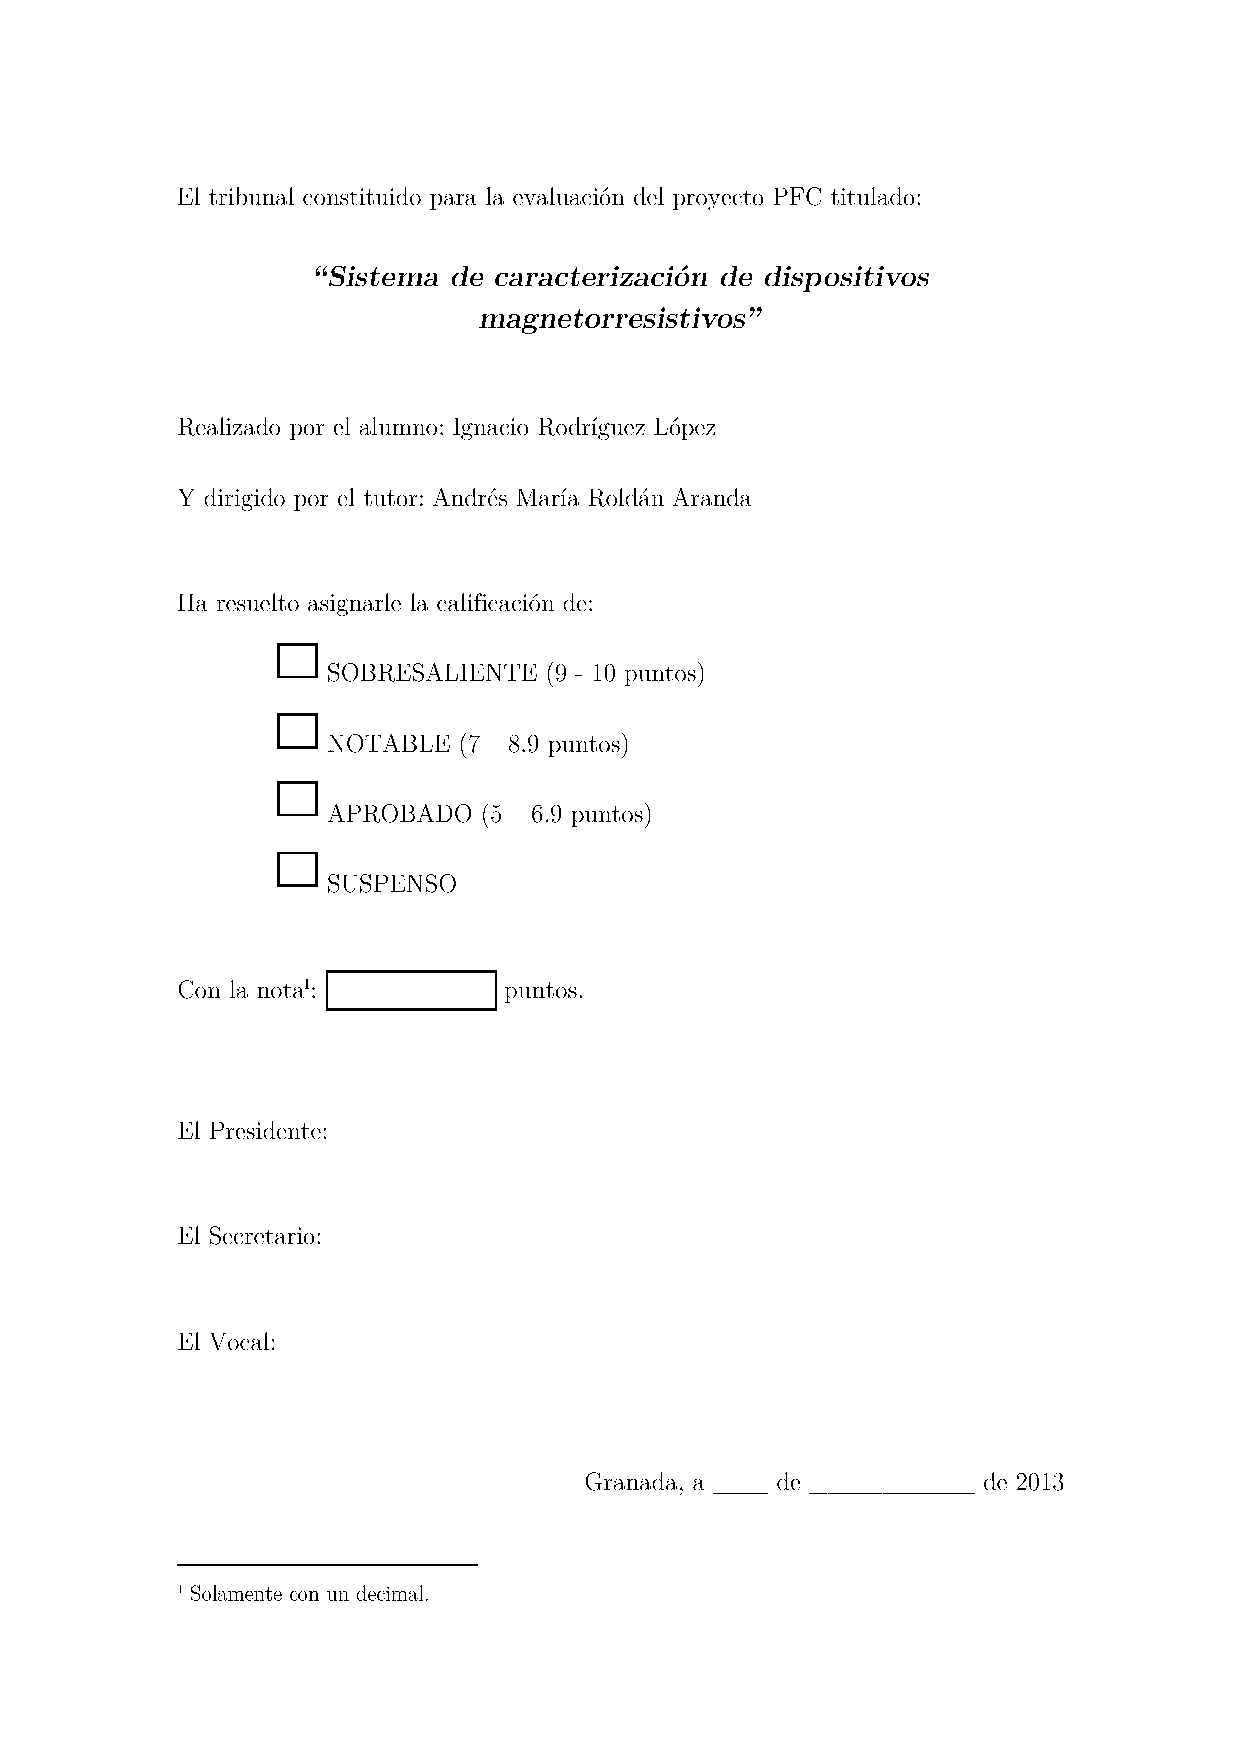
\includepdf[pages=-,link=true,linkname=hojaEvaluacionesUGR]{anexoIV_actaPFC}

\newpage
\thispagestyle{empty}

%Begin ----  Para que funcione bien el TOC en PDF
\cleardoublepage
\thispagestyle{empty}
\phantomsection
\addcontentsline{toc}{chapter}{Autorización Lectura}

\noindent D. Andrés María Roldán Aranda, Profesor del departamento
de Electrónica y Tecnología de los Computadores de la Universidad
de Granada, como director del Proyecto Fin de Carrera de D. Víctor Manuel Fernández Castro,

\vspace*{1cm}

Informa:

\begin{doublespace}
que el presente trabajo, titulado:
\end{doublespace}

\begin{doublespace}
\begin{center}
\textbf{\emph{\large {}``Interpretación remota de partituras sobre instrumentos de viento''}}
\par\end{center}{\large \par}
\end{doublespace}

\noindent ha sido realizado y redactado por el mencionado alumno bajo
nuestra dirección, y con esta fecha autorizo a su presentación. 

\vspace*{1cm}

\begin{center}
%Granada, a 06 de Julio de 2012 
Granada, a ~~~~~~ de Junio de 2015
\par\end{center}

\bigskip%%%%%%%o
\bigskip%%%%%%%o
\begin{doublespace}
\hspace{4cm}Fdo.
\end{doublespace}

\newpage
\thispagestyle{empty}
\noindent

\newpage
\thispagestyle{empty}

~

%Begin ----  Para que funcione bien el TOC en PDF
\cleardoublepage
\phantomsection
\thispagestyle{empty}

\addcontentsline{toc}{chapter}{Autorización Depósito Biblioteca}

\noindent Los abajo firmantes autorizan a que la presente copia de
Proyecto Fin de Carrera se ubique en la Biblioteca del Centro y/o
departamento para ser libremente consultada por las personas que lo
deseen.

\vspace*{1cm}

\begin{center}
%Granada, a 06 de Julio de 2012
Granada, a ~~~~~~ de Agosto de 2015
\par\end{center}

\bigskip%%%%%%%o
\bigskip%%%%%%%o
\begin{doublespace}
\hspace{4cm}Fdo.
\end{doublespace}

\newpage
\thispagestyle{empty}

~

%Begin ----  Para que funcione bien el TOC en PDF
\cleardoublepage
\phantomsection
\thispagestyle{empty}
\addcontentsline{toc}{chapter}{Resumen}

\begin{center}
\textbf{\Large Interpretación remota de partituras sobre instrumentos de viento}
\par\end{center}{\Large \par}

\begin{center}
\textbf{\large Víctor Manuel Fernández Castro}
\par\end{center}{\large \par}

\vspace{0.75cm}






\begin{doublespace}
\noindent \textbf{PALABRAS CLAVE:}
\end{doublespace}



\begin{singlespace}
\noindent Raspberry Pi, Órgano, MIDI, Web, Linux, Demonio, C, PHP, Python, GPIO, Solidworks.

\end{singlespace}

\begin{doublespace}
\noindent \textbf{RESUMEN:}
\end{doublespace}

\begin{singlespace}

\noindent Este proyecto tendrá como objetivo dotar a un sistema mecánico de pulsación del soporte necesario para interpretar partituras musicales para órgano sobre un Raspberry Pi. Comprende la realización de un intérprete de archivos MIDI, un controlador para la salida por GPIO y una interfaz gráfica de usuario web que permita administrar partituras y controlar la reproducción remotamente. Prestaremos especial atención al órgano de la Parroquia de la Encarnación de Santa Fe (Granada).
\end{singlespace}

\vspace{1.25cm}

\begin{doublespace}
\noindent \textbf{KEYWORDS:}
\end{doublespace}

\begin{singlespace}
\noindent Raspberry Pi, Organ, MIDI, Web, Linux, Daemon, C, PHP, Python, GPIO, Solidworks.
\end{singlespace}

\begin{doublespace}
\noindent \textbf{ABSTRACT:}
\end{doublespace}

\begin{singlespace}
\noindent This project will aim to give a mechanical pulsation system the neccesary support to play musical scores for pipe organ on a Raspberry Pi. All this includes the implementation of a MIDI file interpreter, a GPIO output driver and a graphical user interface to manage scores and controlling the playback remotely. We'll pay particular attention to the pipe organ at the Church of Santa Fe (Granada).
\end{singlespace}

\newpage
\thispagestyle{empty}

~

%Begin ----  Para que funcione bien el TOC en PDF
\cleardoublepage
\phantomsection
\thispagestyle{empty}
\addcontentsline{toc}{chapter}{Dedicatoria}

\vspace{6cm}

\begin{quotation}
\noindent \begin{center}
\textbf{\emph{\Large Dedicado a}}\textbf{\emph{\large }}\\
\textbf{\emph{\large }}\\
\textbf{\emph{\large }}\\
\textbf{\emph{\large Mi familia y mis amigos. Por estar siempre ahí.}}
\par\end{center}{\large \par}
\end{quotation}
\newpage
\thispagestyle{empty}

~\newpage
\thispagestyle{empty}


